\documentclass[11pt,oneside]{article}	%use"amsart"insteadof"article"forAMSLaTeXformat
\usepackage{geometry}		%Seegeometry.pdftolearnthelayoutoptions.Therearelots.
\geometry{letterpaper}		%...ora4paperora5paperor...
%\geometry{landscape}		%Activateforforrotatedpagegeometry
%\usepackage[parfill]{parskip}		%Activatetobeginparagraphswithanemptylineratherthananindent
\usepackage{graphicx}				%Usepdf,png,jpg,orepsßwithpdflatex;useepsinDVImode
								%TeXwillautomaticallyconverteps-->pdfinpdflatex		
\usepackage{amssymb}
\usepackage{amsmath}
\usepackage[colorlinks]{hyperref}

%----macros begin---------------------------------------------------------------
\usepackage{color}
\usepackage{amsthm}
\usepackage{amsmath}

\def\conv{\mbox{\textrm{conv}\,}}
\def\aff{\mbox{\textrm{aff}\,}}
\def\E{\mathbb{E}}
\def\R{\mathbb{R}}
\def\Z{\mathbb{Z}}
\def\tex{\TeX}
\def\latex{\LaTeX}
\def\v#1{{\bf #1}}
\def\p#1{{\bf #1}}
\def\T#1{{\bf #1}}

\def\vet#1{{\left(\begin{array}{cccccccccccccccccccc}#1\end{array}\right)}}
\def\mat#1{{\left(\begin{array}{cccccccccccccccccccc}#1\end{array}\right)}}

\def\lin{\mbox{\rm lin}\,}
\def\aff{\mbox{\rm aff}\,}
\def\pos{\mbox{\rm pos}\,}
\def\cone{\mbox{\rm cone}\,}
\def\conv{\mbox{\rm conv}\,}
\newcommand{\homog}[0]{\mbox{\rm homog}\,}
\newcommand{\relint}[0]{\mbox{\rm relint}\,}

%----macros end-----------------------------------------------------------------

\title{Boolean combinations of cellular complexes as chain operations
\footnote{This document is part of the \emph{Linear Algebraic Representation with CoChains} (LAR-CC) framework~\cite{cclar-proj:2013:00}. \today}
}
\author{Alberto Paoluzzi}
%\date{}							%Activatetodisplayagivendateornodate

\begin{document}
\maketitle
\tableofcontents
\nonstopmode

%-------------------------------------------------------------------------------
\section{Introduction}
%-------------------------------------------------------------------------------

In this module a novel approach to Boolean operations of cellular complexes is defined and implemented. The novel algorithm may be summarised as follows. 

First we compute the CDC (Common Delaunay Complex) of the input LAR complexes $A$ and $B$, to get a LAR of the \emph{simplicial} CDC.

Then, we split the cells intersecting the boundary faces of the input complexes, getting the final \emph{polytopal} SCDC  
(Split Common Delaunay Complex), whose cells  provide the  basis for the linear coordinate representation of both input 
complexes, upon the same space decomposition.

Afterwards, every Boolean result is computed by bitwise operations, between the coordinate representations of the transformed $A$ and $B$ input.

Finally a greedy assembly of SCDC cells is executed, in order to return a polytopal complex with a reduced number of cells.



\subsection{Preview of the Boolean algorithm}
%-------------------------------------------------------------------------------

The goal is the computation of $A \diamond B$, with $\diamond\in \{\cup, \cap, -\}$, where a LAR representation of both $A$ and $B$ is given. The Boolean algorithm works as follows.

\begin{enumerate}
\item 
Embed both cellular complexes $A$ and $B$ in the same space (say, identify their common vertices) by $V_{ab} = V_a \cup V_b$.
\item 
Build their CDC  (Common Delaunay Complex) as the LAR of \emph{Delaunay triangulation} of the vertex set $V_{ab}$, and embedded $\partial A$ and $\partial B$ in it.
\item 
Split the (highest-dimensional) cells of CDC crossed by $\partial A$ or $\partial B$. Their lower dimensional faces remain partitioned accordingly. We name the resulting complex SCDC (Split Common Delaunay Complex).
\item 
With respect to the SCDC basis of $d$-cells $C_d$, compute two coordinate chains $\alpha,\beta: C_d \to \{0,1\}$, such that: 
\begin{align}
	\alpha(cell) &= 1  \quad\mbox{if\ } |cell| \subset A;  \quad\mbox{else\ } \alpha(cell) = 0, \nonumber\\
	\beta(cell) &= 1  \quad\mbox{if\ } |cell| \subset B;  \quad\mbox{else\ } \beta(cell) = 0. \nonumber
\end{align}
\item 
Extract accordingly the SCDC chain corresponding to $A \diamond B$, with $\diamond\in \{\cup, \cap, -\}$.
\end{enumerate}


\subsection{Remarks}
%-------------------------------------------------------------------------------

You may  make an analogy between the SCDC (\emph{Split} CDC) and a CDT (Constrained Delaunay Triangulation).  In part they coincide, but in general, the SCDC is a polytopal complex, and is not a simplicial complex as the CDC.

The more complex algorithmic step is the cell splitting.  
Every time, a single $d$-cell  $c$  is split by a single hyperplane (cutting its interior)  giving either two splitted cells $c_1$ and $c_2$, or just one output cell (if the hyperplane is the affine hull of the CDC facet)
whatever the input cell dimension $d$.  After every splitting of the cell interior, the row $c$ is substituted (within the \texttt{CV} matrix) by $c_1$, and $c_2$ is 
added to the end of the \texttt{CV} matrix, as a new row.

The splitting process is started by ``splitting seeds" generated by $(d-1)$-faces of both operand boundaries.
In fact, every such face, say $f$, has vertices on CDC and \emph{may} split some incident CDC $d$-cell.  In particular, starting from its vertices,
$f$ must split the CDC cells in whose interior it passes though.

So, a dynamic data structure is set-up, storing for each boundary face $f$ the list of cells it must cut, and, for every CDC $d$-cell with interior traversed
by some such $f$, the list of cutting faces.  This data structure is continuously updated during the splitting process, using the 
adjacent cells of the split ones, who are to be split in turn.  Every split cell may add some adjacent cell to be split, and after the split,
the used pair (\texttt{cell,face}) is removed.  The splitting process continues until the data structure becomes empty.

Every time a cell is split, it is characterized as either internal (1) or external (0) to the used (oriented) boundary facet f, so that the two 
resulting subcells $c_1$ and $c_2$  receive two opposite characterization (with respect to the considered boundary).

At the very end, every (polytopal) SCDC $d$-cell has two bits of information (one for argument $A$ and one for argument $B$), telling whether it is internal  (1) or external (0) or unknown (-1) with respect to every Boolean argument.

A final recursive traversal of the SCDC, based on cell adjacencies, transforms every $-1$ into either 0 or 1, providing the two final chains to be bitwise operated, depending on the Boolean operation to execute.


%-------------------------------------------------------------------------------
\section{Step 1: merging discrete spaces}
%-------------------------------------------------------------------------------


\subsection{Requirements}
%-------------------------------------------------------------------------------

The \emph{join} of two sets $P, Q \subset \E^d$ is the set $PQ = \{\alpha \v{x} + \beta \v{y}\,| \v{x} \in P,\  \v{y} \in Q\}$,
where $\alpha, \beta \in \R$, $\alpha, \beta \geq 0$, and $\alpha + \beta = 1$. The join operation is associative and commutative.


\paragraph{Input} 
Two LAR models of two non-empty ``solid'' $d$-spaces $A$ and $B$, denoted as \texttt{(V1,CV1)} and \texttt{(V2,CV2)}. 


\paragraph{Output} 
The LAR representation \texttt{(V,CV)} of Delaunay triangulation (simplicial $d$-complex) of the set $\conv AB \subset \E^d$, convex hull of the join of $A$ and $B$, named Common Delaunay Complex (CDC) in the following.

\paragraph{Auxiliary data structures} 
This software module returns also:

\begin{enumerate}
\item 
a dictionary \texttt{vertDict} of \texttt{V} vertices, with \emph{key} the symbolic representation of vertices \texttt{v} returned by expressions \texttt{vcode(v)}, $\texttt{v}\in \texttt{V}$, and with values the finite ordinal numbers of the vertices;

\item 
the numbers \texttt{n1}, \texttt{n12}, \texttt{n2} of the elements of \texttt{V1}, $\texttt{V1}\cap\texttt{V2}$, and \texttt{V2}, respectively. Notice that the following assertions must hold (see Figure~\ref{fig:bounds}):
\begin{align}
\texttt{n1} - \texttt{n12} + \texttt{n2} &= \texttt{n} \\
0 < \texttt{n} - \texttt{n2}  &\leq  \texttt{n1}  <  \texttt{n} 
\end{align}

\item the input boundary complex \texttt{(V,BC)}, with $\texttt{BC} = \texttt{BC1+BC2}$, i.e.~the union of the  two boundary $(d-1)$-complexes \texttt{(V,BC1)} and \texttt{(V,BC2)}, defined on the common vertices.
\end{enumerate}

\begin{figure}[htbp] %  figure placement: here, top, bottom, or page
   \centering
   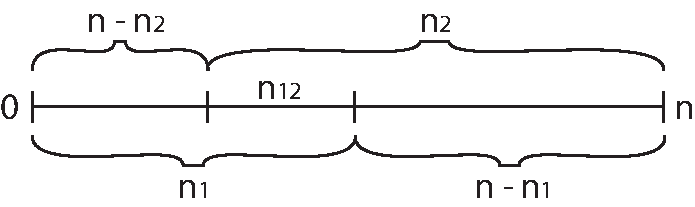
\includegraphics[width=0.5\linewidth]{images/bounds} 
   \caption{Relationships inside the orderings of CDC vertices}
   \label{fig:bounds}
\end{figure}

\subsection{Implementation}
%-------------------------------------------------------------------------------


%-------------------------------------------------------------------------------
@D Compute model boundaries of complex of convex cells
@{""" Compute model boundaries of complex of convex cells """

def larFacetsOfPolytopalComplex(vertDict,cells,facets):
	(V1,CV1),(V2,CV2) = model1,model2
	for cell in CV1:
		Vcell = [V1[v] for v in cell]

@}
%-------------------------------------------------------------------------------


%-------------------------------------------------------------------------------
@D Merge two dictionaries with keys the point locations
@{""" Merge two dictionaries with keys the point locations """
def mergeVertices(model1, model2):

	(V1,CV1),(V2,CV2) = model1, model2

	n = len(V1); m = len(V2)
	def shift(CV, n): 
		return [[v+n for v in cell] for cell in CV]
	CV2 = shift(CV2,n)

	vdict1 = defaultdict(list)
	for k,v in enumerate(V1): vdict1[vcode(v)].append(k) 
	vdict2 = defaultdict(list)
	for k,v in enumerate(V2): vdict2[vcode(v)].append(k+n) 
	vertDict = defaultdict(list)
	for point in vdict1.keys(): vertDict[point] += vdict1[point]
	for point in vdict2.keys(): vertDict[point] += vdict2[point]

	case1, case12, case2 = [],[],[]
	for item in vertDict.items():
		key,val = item
		if len(val)==2:  case12 += [item]
		elif val[0] < n: case1 += [item]
		else: case2 += [item]
	n1 = len(case1); n2 = len(case12); n3 = len(case2)

	invertedindex = list(0 for k in range(n+m))
	for k,item in enumerate(case1):
		invertedindex[item[1][0]] = k
	for k,item in enumerate(case12):
		invertedindex[item[1][0]] = k+n1
		invertedindex[item[1][1]] = k+n1
	for k,item in enumerate(case2):
		invertedindex[item[1][0]] = k+n1+n2

	V = [eval(p[0]) for p in case1] + [eval(p[0]) for p in case12] + [eval(
				p[0]) for p in case2]
	CV1 = [sorted([invertedindex[v] for v in cell]) for cell in CV1]
	CV2 = [sorted([invertedindex[v] for v in cell]) for cell in CV2]

	return V,CV1,CV2, n1+n2,n2,n2+n3
@}
%-------------------------------------------------------------------------------




	
%-------------------------------------------------------------------------------
@D Make Common Delaunay Complex
@{""" Make Common Delaunay Complex """
def makeCDC(arg1,arg2):

	(V1,basis1), (V2,basis2) = arg1,arg2
	(facets1,cells1),(facets2,cells2) = basis1[-2:],basis2[-2:]
	model1, model2 = (V1,cells1),(V2,cells2)

	V, _,_, n1,n12,n2 = mergeVertices(model1, model2)
	n = len(V)
	assert n == n1 - n12 + n2
	
	CV = sorted(AA(sorted)(Delaunay(array(V)).simplices))
	vertDict = defaultdict(list)
	for k,v in enumerate(V): vertDict[vcode(v)] += [k]
	
	BC1 = signedCellularBoundaryCells(V1,basis1)
	BC2 = signedCellularBoundaryCells(V2,basis2)
	BC = [[ vertDict[vcode(V1[v])][0] for v in cell] for cell in BC1] + [ 
			[ vertDict[vcode(V2[v])][0] for v in cell] for cell in BC2]
	
	return V,CV,vertDict,n1,n12,n2,BC
@}
%-------------------------------------------------------------------------------




%-------------------------------------------------------------------------------
\section{Step 2: splitting cells}
%-------------------------------------------------------------------------------

The goal of this section is to transform the CDC simplicial complex, into the polytopal Split Common Delaunay Complex (SCDC), by splitting the $d$-cells of CDC crossed in their interior by some cell of the input boundary complex.

\subsection{Requirements}
%-------------------------------------------------------------------------------
We call here for a sequential implementation, following every $(d-1)$-facet \texttt{lambda} in \texttt{BC} (for \emph{Boundary Cells}). We start the splitting with \texttt{COVECTOR(lambda)} from \texttt{cell}, one of the CDC $d$-cells  incident on a vertex of \texttt{lambda}, and continue the splitting on the $d$-cells $(d-1)$-adjacent  to \texttt{cell}, where (a) \texttt{COVECTOR(lambda)} either crosses the \texttt{cell}'s interior or contains one of \texttt{cell}'s $(d-1)$-facets \and{and} (b) such that the intersection with \texttt{lambda} is not empty, until the queue (or stack) of $d$-cells to intersect with \texttt{covector} is not empty.

\paragraph{Best computational strategy}
First associate to each cutting facet the list of cells it may cut; then execute all the cuts. In this way we can compute the adjacency matrix just one time at the beginning of the procedure, and do not need to update it after every split.

\paragraph{Input}
The output of previous algorithm stage.

\paragraph{Output}
The LAR representation \texttt{(W,PW)} of the SCDC,

\paragraph{Auxiliary data structures} 
This software module returns also
 a dictionary \texttt{splitFacets}, with keys the  input boundary faces and values the list of pairs\texttt{(covector,fragmentedFaces)}.   


\subsection{Implementation}
%-------------------------------------------------------------------------------


\paragraph{Computing the adjacent cells of a given cell}
To perform this task we make only use of the \texttt{CV} list. In a more efficient implementation we should make direct use of the sparse adjacency matrix, to be dynamically updated together with the \texttt{CV} list.
The computation of the adjacent $d$-cells of a single $d$-cell is given here by extracting a column of the $\texttt{CSR}(M_d\, M_d^t)$. This can be done by multiplying $\texttt{CSR}(M_d)$ by its transposed row corresponding to the query $d$-cell. 

%-------------------------------------------------------------------------------
@D Computing the adjacent cells of a given cell
@{""" Computing the adjacent cells of a given cell """
def adjacencyQuery (V,CV):
	dim = len(V[0])
	def adjacencyQuery0 (cell):
		nverts = len(CV[cell])
		csrCV =  csrCreate(CV)
		csrAdj = matrixProduct(csrCV,csrTranspose(csrCV))
		cellAdjacencies = csrAdj.indices[csrAdj.indptr[cell]:csrAdj.indptr[cell+1]]
		return [acell for acell in cellAdjacencies if dim <= csrAdj[cell,acell] < nverts]
	return adjacencyQuery0
@}
%-------------------------------------------------------------------------------

\paragraph{Updating the adjacency matrix}
At every step of the CDC splitting, generating two output cells \texttt{cell1} and  \texttt{cell2} from the input  \texttt{cell}, the element of such index in the list \texttt{CV} is restored with the \texttt{cell1} vertices, and a new (last) element is created in \texttt{CV}, to store the \texttt{cell2} vertices.
Therefore the row of index \texttt{cell} of the symmetric  adjacency matrix must be recomputed, being the \texttt{cell} column updated consequently. Also, a new last row (and column) must be added to the matrix. 

%-------------------------------------------------------------------------------
@D Updating the adjacency matrix
@{""" Updating the adjacency matrix """
pass
@}
%-------------------------------------------------------------------------------



\paragraph{Relational inversion (characteristic matrix transposition)}

The operation could be executed by simple matrix transposition of the CSR (Compressed Sparse Row) representation of the sparse characteristic matrix $M_d \equiv \texttt{CV}$.
A simple relational inversion using Python lists is given here. The \texttt{invertRelation} function 
is given here, linear in the size of the \texttt{CV} list, where the complexity of each cell is constant and 
small in most cases.

%-------------------------------------------------------------------------------
@D Characteristic matrix transposition
@{""" Characteristic matrix transposition """
def invertRelation(CV):
	columnNumber = max(AA(max)(CV))+1
	VC = [[] for k in range(columnNumber)]
	for k,cell in enumerate(CV):
		for v in cell:
			VC[v] += [k]
	return VC
@}
%-------------------------------------------------------------------------------


\paragraph{Computation of splitting tests}

In order to compute, in the simplest and more general way, whether each of the two split $d$-cells is internal or external to the splitting boundary $d-1$-facet, it is necessary to consider the oriented covector $\phi$ (or one-form) canonically associated to the facet $f$ by the covector representation theorem, i.e.~the corresponding oriented hyperplane. In this case, the internal/external attribute of the split cell will be computed by evaluating the pairing $<v,\phi>$.

%-------------------------------------------------------------------------------
@D Splitting tests
@{""" Splitting tests """
def testingSubspace(V,covector):
	def testingSubspace0(vcell):
		inout = SIGN(sum([INNERPROD([[1.]+V[v],covector]) for v in vcell]))
		return inout
	return testingSubspace0
	
def cuttingTest(covector,polytope,V):
	signs = [INNERPROD([covector, [1.]+V[v]]) for v in polytope]
	signs = eval(vcode(signs))
	return any([value<-0.001 for value in signs]) and any([value>0.001 for value in signs])
	
def tangentTest(covector,facet,adjCell,V):
	common = list(set(facet).intersection(adjCell))
	signs = [INNERPROD([covector, [1.]+V[v]]) for v in common]
	count = 0
	for value in signs:
		if -0.0001<value<0.0001: count +=1
	if count >= len(V[0]): 
		return True
	else: 
		return False	
@}
%-------------------------------------------------------------------------------




\paragraph{Elementary splitting test}

Let us remember that the adjacency matrix between $d$-cells is computed via SpMSpM multiplication by the double application 
\[
\texttt{adjacencyQuery(V,CV)(cell)}, 
\] 
where the first application \texttt{adjacencyQuery(V,CV)}
returns a partial function with bufferisation of the adjacency matrix, and the second application to \texttt{cell} returns the list of adjacent $d$-cells sharing with it a $(d-1)$-dimensional facet.

%-------------------------------------------------------------------------------
@D Elementary splitting test
@{
@< Splitting tests @>

""" Elementary splitting test """
def dividenda(V,CV, cell,facet,covector,unchosen):
	out = []
	adjCells = adjacencyQuery(V,CV)(cell)
	for adjCell in set(adjCells).difference(unchosen):
		if (cuttingTest(covector,CV[adjCell],V) and \
			cellFacetIntersecting(facet,adjCell,covector,V,CV)) or \
			tangentTest(covector,facet,CV[adjCell],V): out += [adjCell]
	return out
@}
%-------------------------------------------------------------------------------

\paragraph{CDC cell splitting with one or more facets}

%-------------------------------------------------------------------------------
@D CDC cell splitting with one or more cutting facets
@{""" CDC cell splitting with one or more cutting facets """
def fragment(cell,cellCuts,V,CV,BC):
	vcell = CV[cell]
	cellFragments = [[V[v] for v in vcell]]
	
	for f in cellCuts[cell]:
		facet = BC[f]
		plane = COVECTOR([V[v] for v in facet])
		for k,fragment in enumerate(cellFragments):
		
    		#if not tangentTest(plane,facet,fragment,V):
			[below,equal,above] = SPLITCELL(plane,fragment)
			if below != above:
				cellFragments[k] = below
				cellFragments += [above]
	
	return cellFragments
@}
%-------------------------------------------------------------------------------

\paragraph{SCDC splitting with every boundary facet}
The function \texttt{makeSCDC} is used  to compute the LAR model \texttt{(W,CW)} of the SCDC.
It takes as input the LAR model \texttt{(V,CV)} of the CDC, and the LAR model \texttt{(V,BC)} of the input Boolean Complex, and returns also the vertex-cell relation \texttt{VC}, i.e.~the transposed of \texttt{CV}.

For every $\texttt{k} \in \texttt{BC}$, a list \texttt{cellsToSplit}

%-------------------------------------------------------------------------------
@D SCDC splitting with every boundary facet
@{""" SCDC splitting with every boundary facet """
def makeSCDC(V,CV,BC):
	index = -1
	defaultValue = -1
	VC = invertRelation(CV)
	CW = []
	Wdict = dict()
	BCellcovering = boundaryCover(V,CV,BC,VC)
	cellCuts = invertRelation(BCellcovering)
	for k in range(len(CV) - len(cellCuts)): cellCuts += [[]]
	
	for k,frags in enumerate(cellCuts):
		if cellCuts[k] == []:
			cell = []
			for v in CV[k]:
				key = vcode(V[v])
				if Wdict.get(key,defaultValue) == defaultValue:
					index += 1
					Wdict[key] = index
					cell += [index]
				else: 
					cell += [Wdict[key]]
			CW += [cell]
		else:
			cellFragments = fragment(k,cellCuts,V,CV,BC)
			for cellFragment in cellFragments:
				cellFrag = []
				for v in cellFragment:
					key = vcode(v)
					if Wdict.get(key,defaultValue) == defaultValue:
						index += 1
						Wdict[key] = index
						cellFrag += [index]
					else: 
						cellFrag += [Wdict[key]]
				CW += [cellFrag]
	W = sorted(zip( Wdict.values(), Wdict.keys() ))
	W = AA(eval)(TRANS(W)[1])
	return W,CW,VC,BCellcovering,cellCuts
@}
%-------------------------------------------------------------------------------

\paragraph{Computation of boundary facets covering with CDC cells}

%-------------------------------------------------------------------------------
@D Computation of boundary facets covering with CDC cells
@{""" Computation of boundary facets covering with CDC cells """
def boundaryCover(V,CV,BC,VC):
	cellsToSplit = list()
	boundaryCellCovering = []
	for k,facet in enumerate(BC):
		covector = COVECTOR([V[v] for v in facet])
		seedsOnFacet = VC[facet[0]]
		cellsToSplit = [dividenda(V,CV, cell,facet,covector,[]) for cell in seedsOnFacet ]
		cellsToSplit = set(CAT(cellsToSplit))
		while True:
			newCells = [dividenda(V,CV, cell,facet,covector,cellsToSplit) for cell in cellsToSplit ]
			if newCells != []: newCells = CAT(newCells)
			covering = cellsToSplit.union(newCells)
			if covering == cellsToSplit: 
    			break
			cellsToSplit = covering
		boundaryCellCovering += [list(covering)]
	return boundaryCellCovering
@}
%-------------------------------------------------------------------------------

\paragraph{Cell-facet intersection test}

%-------------------------------------------------------------------------------
@D Cell-facet intersection test
@{""" Cell-facet intersection test """
def cellFacetIntersecting(boundaryFacet,cell,covector,V,CV):
	points = [V[v] for v in CV[cell]]
	vcell1,newFacet,vcell2 = SPLITCELL(covector,points,tolerance=1e-4,ntry=4)
	boundaryFacet = [V[v] for v in boundaryFacet]
	translVector = boundaryFacet[0]
	
	# translation 
	newFacet = [ VECTDIFF([v,translVector]) for v in newFacet ]
	boundaryFacet = [ VECTDIFF([v,translVector]) for v in boundaryFacet ]
	
	# linear transformation: boundaryFacet -> standard (d-1)-simplex
	d = len(V[0])
	transformMat = mat( boundaryFacet[1:d] + [covector[1:]] ).T.I
	
	# transformation in the subspace x_d = 0
	newFacet = (transformMat * (mat(newFacet).T)).T.tolist()
	boundaryFacet = (transformMat * (mat(boundaryFacet).T)).T.tolist()
	
	# projection in E^{d-1} space and Boolean test
	newFacet = MKPOL([ AA(lambda v: v[:-1])(newFacet), [range(1,len(newFacet)+1)], None ])
	boundaryFacet = MKPOL([ AA(lambda v: v[:-1])(boundaryFacet), [range(1,len(boundaryFacet)+1)], None ])
	verts,cells,pols = UKPOL(INTERSECTION([newFacet,boundaryFacet]))
	
	if verts == []: return False
	else: return True
@}
%-------------------------------------------------------------------------------








%-------------------------------------------------------------------------------
\section{Step 3: cell labeling}
%-------------------------------------------------------------------------------

The goal of this stage is to label every cell of the SCDC with two bits, corresponding to the input spaces $A$ and $B$, and telling whether the cell is either internal (1) or external (0) to either spaces.

\subsection{Requirements}
%-------------------------------------------------------------------------------


\paragraph{Input}
The output of previous algorithm stage.

\paragraph{Output}
The array \texttt{cellLabels} with \emph{shape} $\texttt{len(PW)}\times 2$, and values in $\{0,1\}$.

\section{Step 4: greedy cell gathering}

The goal of this stage is to make as lower as possible the number of cells in the  output LAR of the space $AB$, partitioned into convex cells.

\paragraph{Input}
The LAR model \texttt{(W,PW)} of the SCDC and the array \texttt{cellLabels}.

\paragraph{Output}
The LAR representation \texttt{(W,RW)} of the final fragmented and labeled space $AB$.


%-------------------------------------------------------------------------------
\section{Exporting the library}
%-------------------------------------------------------------------------------


%-------------------------------------------------------------------------------
@O lib/py/bool1.py
@{""" Module for Boolean ops with LAR """
@< Initial import of modules @>
DEBUG = False
from splitcell import *
@< Merge two dictionaries with keys the point locations @>
@< Make Common Delaunay Complex @>
@< Cell-facet intersection test @>
@< Elementary splitting test @>
@< Computing the adjacent cells of a given cell @>
@< Computation of boundary facets covering with CDC cells @>
@< CDC cell splitting with one or more cutting facets @>
@< SCDC splitting with every boundary facet @>
@< Characteristic matrix transposition @>
@}
%-------------------------------------------------------------------------------

%-------------------------------------------------------------------------------
\section{Tests and examples}
%-------------------------------------------------------------------------------

%-------------------------------------------------------------------------------
@D Debug input and vertex merging
@{
V1,basis1 = arg1
V2,basis2 = arg2
cells1 = basis1[-1]
cells2 = basis2[-1]

if DEBUG: VIEW(STRUCT(MKPOLS((V1,basis1[1])) + MKPOLS((V2,basis2[1]))))

model1,model2 = (V1,cells1),(V2,cells2)
V, CV1,CV2, n1,n12,n2 = mergeVertices(model1,model2)	#<<<<<<<<<<<<<<<<

submodel = SKEL_1(STRUCT(MKPOLS((V,CV1+CV2)))) 
VV = AA(LIST)(range(len(V)))
if DEBUG: VIEW(STRUCT([ submodel,larModelNumbering(V,[VV,_,CV1+CV2],submodel,3)]))

V,CV,vertDict,n1,n12,n2,BC = makeCDC(arg1,arg2)		#<<<<<<<<<<<<<<<<

W,CW,VC,BCellCovering,cellCuts = makeSCDC(V,CV,BC)
assert len(VC) == len(V) 
assert len(BCellCovering) == len(BC)

submodel = STRUCT([ SKEL_1(STRUCT(MKPOLS((V,CV)))), COLOR(RED)(STRUCT(MKPOLS((V,BC)))) ])
dim = len(V[0])
VIEW(STRUCT([ submodel,larModelNumbering(V,[VV,BC,CV],submodel,3)]))
VIEW(EXPLODE(1.2,1.2,1.2)(MKPOLS((W,CW))))
"""
for k in range(1,len(CW)+1):
	VIEW(STRUCT([ STRUCT(MKPOLS((W,CW[:k]))), submodel,larModelNumbering(V,[VV,BC,CV],submodel,3) ]))
"""
@}
%-------------------------------------------------------------------------------


%-------------------------------------------------------------------------------
@O test/py/bool1/test1.py
@{
import sys
""" import modules from larcc/lib """
sys.path.insert(0, 'lib/py/')
from bool1 import *

""" Definition of Boolean arguments """
V1 = [[3,0],[11,0], [13,10], [10,11], [8,11], [6,11], [4,11], [1,10], [4,3], [6,4], 
	[8,4], [10,3]]
FV1 = [[0,1,8,9,10,11],[1,2,11], [3,10,11], [4,5,9,10], [6,8,9], [0,7,8], [2,3,11],
	[3,4,10], [5,6,9], [6,7,8]]
EV1 = [[0,1],[0,7],[0,8],[1,2],[1,11],[2,3],[2,11],[3,4],[3,10],[3,11],[4,5],[4,10],[5,6],[5,9],[6,7],[6,8],[6,9],[7,8],[8,9],[9,10],[10,11]]
VV1 = AA(LIST)(range(len(V1)))

V2 = [[0,3],[14,2], [14,5], [14,7], [14,11], [0,8], [3,7], [3,5]]
FV2 =[[0,5,6,7], [0,1,7], [4,5,6], [2,3,6,7], [1,2,7], [3,4,6]]
EV2 = [[0,1],[0,5],[0,7],[1,2],[1,7],[2,3],[2,7],[3,4],[3,6],[4,5],[4,6],[5,6],[6,7]]
VV2 = AA(LIST)(range(len(V2)))

arg1 = V1,(VV1,EV1,FV1)
arg2 = V2,(VV2,EV2,FV2)
@< Debug input and vertex merging @>
@}
%-------------------------------------------------------------------------------

%-------------------------------------------------------------------------------
@O test/py/bool1/test2.py
@{
import sys
""" import modules from larcc/lib """
sys.path.insert(0, 'lib/py/')
from bool1 import *

V1 = [[3,0],[11,0], [13,10], [10,11], [8,11], [6,11], [4,11], [1,10], [4,3], [6,4], 
	[8,4], [10,3]]
	
FV1 = [[0,1,8,9,10,11],[1,2,11], [3,10,11], [4,5,9,10], [6,8,9], [0,7,8]]
EV1 = [[0,1],[0,7],[0,8],[1,2],[1,11],[2,11],[3,10],[3,11],[4,5],[4,10],[5,9],[6,8],[6,9],[7,8],[8,9],[9,10],[10,11]]
VV1 = AA(LIST)(range(len(V1)))

V2 = [[0,3],[14,2], [14,5], [14,7], [14,11], [0,8], [3,7], [3,5]]
FV2 =[[0,5,6,7], [0,1,7], [4,5,6], [2,3,6,7], [1,2,7], [3,4,6]]
EV2 = [[0,1],[0,5],[0,7],[1,2],[1,7],[2,3],[2,7],[3,4],[3,6],[4,5],[4,6],[5,6],[6,7]]
VV2 = AA(LIST)(range(len(V2)))

arg1 = V1,(VV1,EV1,FV1)
arg2 = V2,(VV2,EV2,FV2)
@< Debug input and vertex merging @>
@}
%-------------------------------------------------------------------------------

%-------------------------------------------------------------------------------
@O test/py/bool1/test3.py
@{
import sys
""" import modules from larcc/lib """
sys.path.insert(0, 'lib/py/')
from bool1 import *

V1 = [[3,0],[11,0], [13,10], [10,11], [8,11], [6,11], [4,11], [1,10], [4,3], [6,4], 
	[8,4], [10,3]]
	
FV1 = [[0,1,8,9,10,11],[1,2,11], [3,10,11], [4,5,9,10], [6,8,9], [0,7,8]]
EV1 = [[0,1],[0,7],[0,8],[1,2],[1,11],[2,11],[3,10],[3,11],[4,5],[4,10],[5,9],[6,8],[6,9],[7,8],[8,9],[9,10],[10,11]]
VV1 = AA(LIST)(range(len(V1)))

V2 = [[0,3],[14,2], [14,5], [14,7], [14,11], [0,8], [3,7], [3,5]]
FV2 =[[0,5,6,7], [0,1,7], [4,5,6], [2,3,6,7]]
EV2 = [[0,1],[0,5],[0,7],[1,7],[2,3],[2,7],[3,6],[4,5],[4,6],[5,6],[6,7]]
VV2 = AA(LIST)(range(len(V2)))

arg1 = V1,(VV1,EV1,FV1)
arg2 = V2,(VV2,EV2,FV2)
@< Debug input and vertex merging @>
@}
%-------------------------------------------------------------------------------


%-------------------------------------------------------------------------------
@O test/py/bool1/test4.py
@{
import sys
""" import modules from larcc/lib """
sys.path.insert(0, 'lib/py/')
from bool1 import *

V1 = [[0,0],[10,0],[10,10],[0,10]]
FV1 = [range(4)]
EV1 = [[0,1],[1,2],[2,3],[0,3]]
VV1 = AA(LIST)(range(len(V1)))

V2 = [[2.5,2.5],[12.5,2.5],[12.5,12.5],[2.5,12.5]]
FV2 = [range(4)]
EV2 = [[0,1],[1,2],[2,3],[0,3]]
VV2 = AA(LIST)(range(len(V2)))

arg1 = V1,(VV1,EV1,FV1)
arg2 = V2,(VV2,EV2,FV2)
@< Debug input and vertex merging @>
@}
%-------------------------------------------------------------------------------

%-------------------------------------------------------------------------------
@O test/py/bool1/test5.py
@{
import sys
""" import modules from larcc/lib """
sys.path.insert(0, 'lib/py/')
from bool1 import *

V1 = [[0,0],[5,0],[5,5],[0,5]]
FV1 = [range(4)]
EV1 = [[0,1],[1,2],[2,3],[0,3]]
VV1 = AA(LIST)(range(len(V1)))

V2 = [[5,0],[10,0],[10,5],[5,5]]
FV2 = [range(4)]
EV2 = [[0,1],[1,2],[2,3],[0,3]]
VV2 = AA(LIST)(range(len(V2)))

arg1 = V1,(VV1,EV1,FV1)
arg2 = V2,(VV2,EV2,FV2)
@< Debug input and vertex merging @>
@}
%-------------------------------------------------------------------------------

%-------------------------------------------------------------------------------
@O test/py/bool1/test6.py
@{
import sys
""" import modules from larcc/lib """
sys.path.insert(0, 'lib/py/')
from bool1 import *

V1 = [[0,0,0],[10,0,0],[10,10,0],[0,10,0],[0,0,10],[10,0,10],[10,10,10],[0,10,10]]
V1,[VV1,EV1,FV1,CV1] = larCuboids((1,1,1),True)
V1 = [SCALARVECTPROD([5,v]) for v in V1]

V2 = [SUM([v,[2.5,2.5,2.5]]) for v in V1]
[VV2,EV2,FV2,CV2] = [VV1,EV1,FV1,CV1]

arg1 = V1,(VV1,EV1,FV1,CV1)
arg2 = V2,(VV2,EV2,FV2,CV2)
@< Debug input and vertex merging @>
@}
%-------------------------------------------------------------------------------

%-------------------------------------------------------------------------------
@O test/py/bool1/test7.py
@{
import sys
""" import modules from larcc/lib """
sys.path.insert(0, 'lib/py/')
from bool1 import *


V1 = [[0,0],[10,0],[10,10],[0,10]]
FV1 = [range(4)]
EV1 = [[0,1],[1,2],[2,3],[0,3]]
VV1 = AA(LIST)(range(len(V1)))

V2 = [[2.5,2.5],[7.5,2.5],[7.5,7.5],[2.5,7.5]]
FV2 = [range(4)]
EV2 = [[0,1],[1,2],[2,3],[0,3]]
VV2 = AA(LIST)(range(len(V2)))

arg1 = V1,(VV1,EV1,FV1)
arg2 = V2,(VV2,EV2,FV2)
@< Debug input and vertex merging @>
@}
%-------------------------------------------------------------------------------

%-------------------------------------------------------------------------------
@O test/py/bool1/test8.py
@{
import sys
""" import modules from larcc/lib """
sys.path.insert(0, 'lib/py/')
from bool1 import *


n = 48
V1 = [[5*cos(angle*2*PI/n)+2.5, 5*sin(angle*2*PI/n)+2.5] for angle in range(n)]
FV1 = [range(n)]
EV1 = TRANS([range(n),range(1,n+1)]); EV1[-1] = [0,n-1]
VV1 = AA(LIST)(range(len(V1)))

V2 = [[4*cos(angle*2*PI/n), 4*sin(angle*2*PI/n)] for angle in range(n)]
FV2 = [range(n)]
EV2 = EV1
VV2 = AA(LIST)(range(len(V2)))

arg1 = V1,(VV1,EV1,FV1)
arg2 = V2,(VV2,EV2,FV2)
@< Debug input and vertex merging @>
@}
%-------------------------------------------------------------------------------

%-------------------------------------------------------------------------------
@O test/py/bool1/test9.py
@{
import sys
""" import modules from larcc/lib """
sys.path.insert(0, 'lib/py/')
from bool1 import *

V1 = [[0,0],[15,0],[15,14],[0,14]]
FV1 = [range(4)]
EV1 = [[0,1],[1,2],[2,3],[0,3]]
VV1 = AA(LIST)(range(len(V1)))

V2 = [[1,1],[7,1],[7,6],[1,6], [8,1],[14,1],[14,7],[8,7], [1,7],[7,7],[7,13],[1,13], [8,8],[14,8],[14,13],[8,13]]
FV2 = [range(4),range(4,8),range(8,12),range(12,16)]
EV2 = [[0,1],[1,2],[2,3],[0,3], [4,5],[5,6],[6,7],[4,7], [8,9],[9,10],[10,11],[8,11], [12,13],[13,14],[14,15],[12,15]]
VV2 = AA(LIST)(range(len(V2)))

arg1 = V1,(VV1,EV1,FV1)
arg2 = V2,(VV2,EV2,FV2)
@< Debug input and vertex merging @>
@}
%-------------------------------------------------------------------------------






%>>>>>>>>>>>>>>>>>>>>>>>>>>>>>>>>>>>>>>>>>>>>>>>>>>>>>>>>>>>>>>>>>>>>>>>>>>>>>>>
\appendix
%>>>>>>>>>>>>>>>>>>>>>>>>>>>>>>>>>>>>>>>>>>>>>>>>>>>>>>>>>>>>>>>>>>>>>>>>>>>>>>>
%-------------------------------------------------------------------------------
\section{Appendix: utility functions}
%-------------------------------------------------------------------------------
@D Initial import of modules
@{from pyplasm import *
from scipy import *
import sys
""" import modules from larcc/lib """
sys.path.insert(0, 'lib/py/')
from lar2psm import *
from simplexn import *
from larcc import *
from largrid import *
from myfont import *
from mapper import *
@}
%------------------------------------------------------------------
\subsection{Numeric utilities}

A small set of utility functions is used to transform a \emph{point} representation, given as array of coordinates, into a string of fixed format to be used as point key into python dictionaries.

%------------------------------------------------------------------
@D Symbolic utility to represent points as strings
@{""" TODO: use package Decimal (http://docs.python.org/2/library/decimal.html) """
global PRECISION
PRECISION = 4.95

def verySmall(number): return abs(number) < 10**-(PRECISION/1.15)

def prepKey (args): return "["+", ".join(args)+"]"

def fixedPrec(value):
	out = round(value*10**(PRECISION*1.1))/10**(PRECISION*1.1)
	if out == -0.0: out = 0.0
	return str(out)
	
def vcode (vect): 
	"""
	To generate a string representation of a number array.
	Used to generate the vertex keys in PointSet dictionary, and other similar operations.
	"""
	return prepKey(AA(fixedPrec)(vect))
@}
%------------------------------------------------------------------


\bibliographystyle{amsalpha}
\bibliography{bool1}

\end{document}
